\section{Evaluation}
    \label{sec:evaluation}
    \begin{figure*}
        \centering
        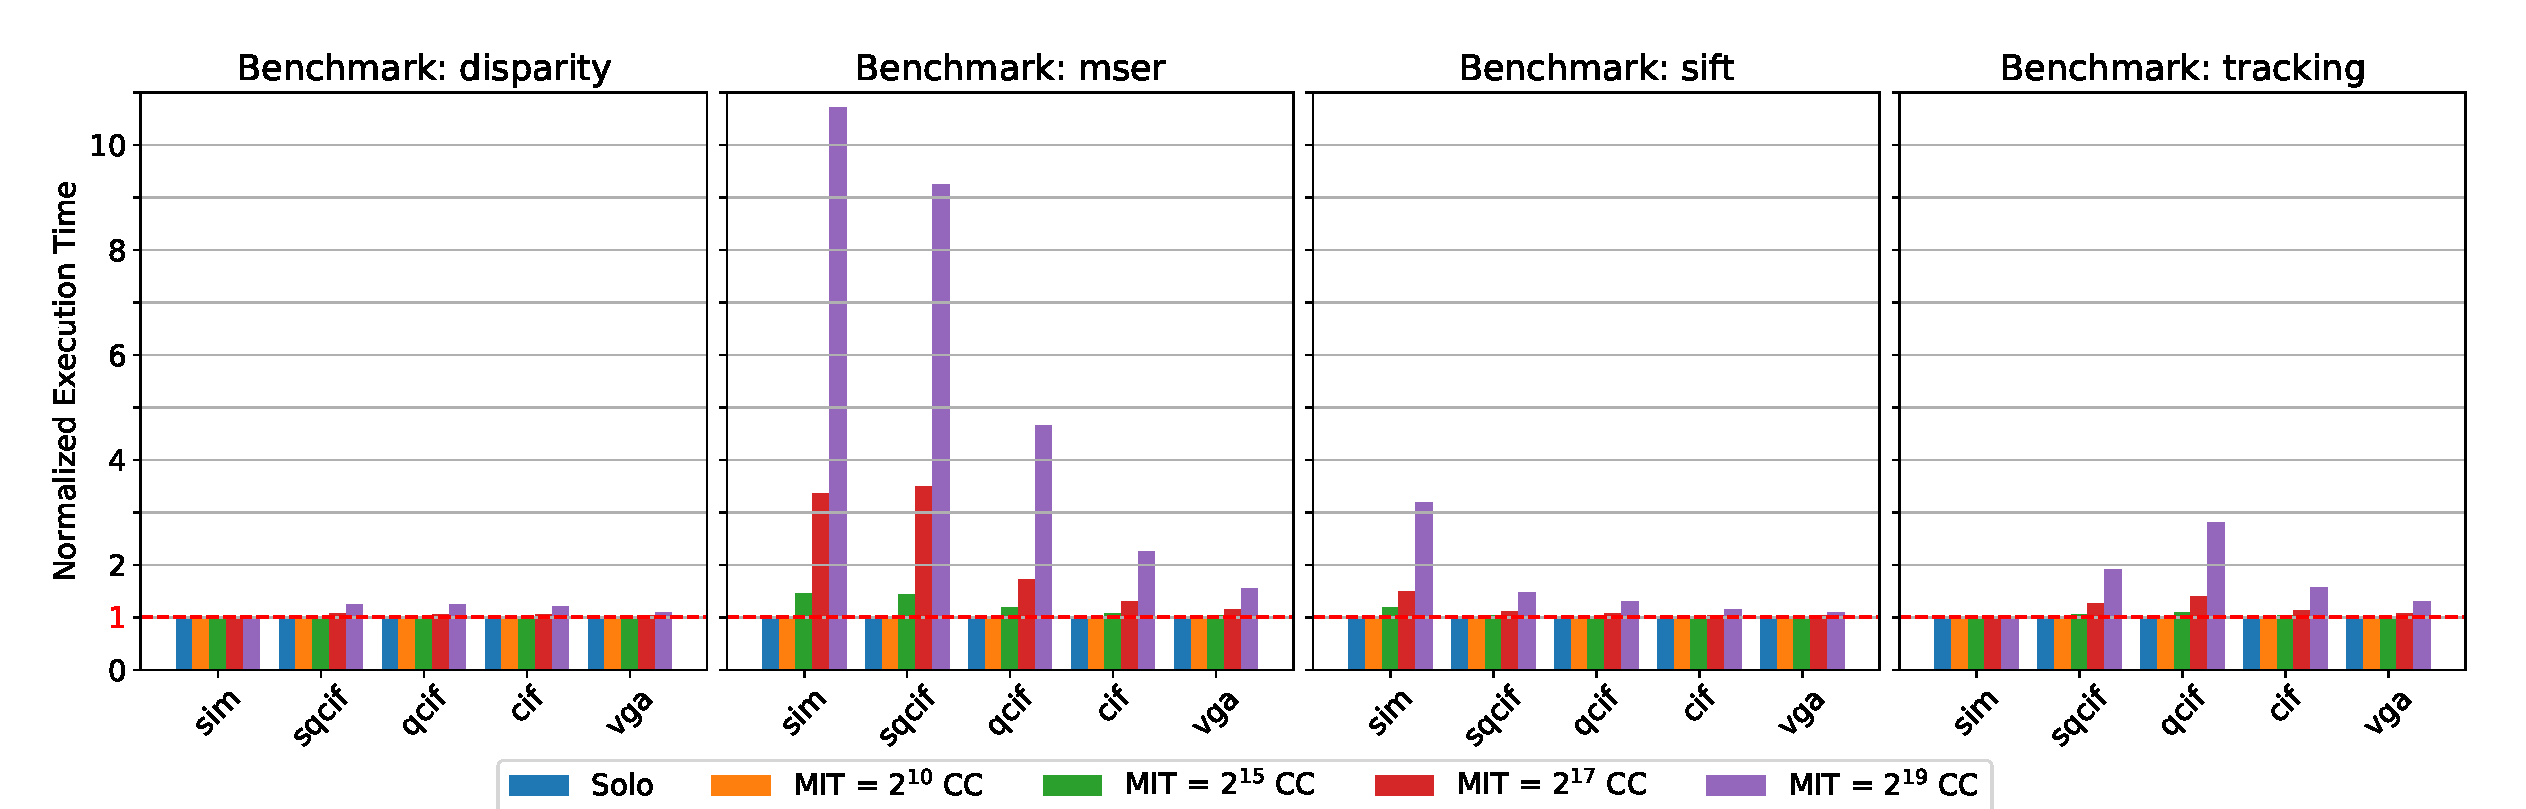
\includegraphics[scale=0.425]{images/cpu-brainfreeze-interference.pdf}
        \caption{Normailized execution time for different combinations of benchmark (inset), input sizes (x axis) and MITs (bar).}
        \label{fig:cpu-brainfreeze-interference-results}
    \end{figure*}

%    For our experiments, we use the Xilinx ZCU102 development board \cite{Xilinx-ULTRASCALE-TRM}, a PS-PL platform featuring four ARM Cortex-A53 cores \cite{ARM-cortex-A53} connected to a shared LLC of 1 MB.
%    Thanks to the Jailhouse hypervisor \cite{ewarp2020rtss}, we are able to isolate the actors by assigning them specific cores and private partitions of the LLC.
%    The victim is allocated three cores and half of the LLC.
%    It runs a selection of benchmarks issued from the San-Diego Vision Benchmark Suite \cite{SD-VBS} on top of Linux 4.14.
%    The attacker is a lightweight bare-metal inmate running on the remaining core.
%    Finally, the PL side and the AXI-Resistor are clocked at 250 MHz.\\
%
%    Following the scenario and setup presented in Section \ref{sec:system_model}, we aim at observing the interference caused by the lightweight attacker on the victim inmate.
%    To this end, we run the selected set of benchmarks for all the available input sizes\footnote{with the exception of \texttt{sim\_fast} and \texttt{full\_hd}} ($x$ axis in Figure \ref{fig:cpu-brainfreeze-interference-results}) and different configurations of the AXI-Resistor (i.e. with MITs of $2^{10}$, $2^{15}$, $2^{17}$ and $2^{19}$).
%    As a baseline, the benchmarks have also been run alone (i.e. without an attacker).
%    This baseline is referred to as "Solo" in Figure \ref{fig:cpu-brainfreeze-interference-results}.
%    All the results for the benchmarks (\texttt{disparity}, \texttt{mser}, \texttt{sift} and \texttt{tracking}) with varying input size have been normalized with respect to the equivalent combination running alone (i.e., Solo the leftmost blue bar in each bar cluster).
%
%    From the results displayed in Figure \ref{fig:cpu-brainfreeze-interference-results}, two oberservations can be made.
%    Firstly, the benchmarks have different sensitivity to the attacker. In fact, it is clear that the \texttt{mser} benchmark is more affected by the attacker than \texttt{disparity}.
%    The former particularly suffers for a small input size (i.e. \texttt{sim}), with its execution time increased by a factor of 10.
%    On the other hand, disparity seems unaffected by the attacker, meaning that spacial isolation of the core is enough.
%    The increments of execution time observed in this experiment are in the same range as those reported by previous research.
%    However, in our case, this interference is caused by only one oustanding memory transaction instead of a continuous flow of transactions generated by 3 cores.
%    Secondly, big MITs tend to introduce more inter-core interference than their counterpart. For instance, a MIT of $2^{19}$ always introduces some visible interference, with varying magnitude.
%
%    Simulating an infinite MIT by configuring the AXI-Resistor such that it accepts the transaction, but never answers systematically leads the whole system to be suspended indefinitely.
%    In other words, if a task tries to fetch data from a non-responding memory, not only its core stalls, but the whole core cluster is suspended.
%    This suggests that for extremely big MITs, significant increases in execution could be observed and that, unlike results in Figure \ref{fig:cpu-brainfreeze-interference-results} such as \texttt{disparity}, tasks deployed on all the cores might be affected by the inter-core interference.

%    For our experiments, we use the Xilinx ZCU102 development board \cite{Xilinx-ULTRASCALE-TRM}, a PS-PL platform featuring four ARM Cortex-A53 cores \cite{ARM-cortex-A53} connected to a shared LLC of 1 MB.
%    Thanks to the Jailhouse-RT project \cite{ewarp2020rtss}, we are able to isolate the actors by assigning them a specific set of cores and a private partition of the LLC.
%    The victim is allocated three cores and half of the LLC.
%    It runs a selection of benchmarks issued from the San-Diego Vision Benchmark Suite \cite{SD-VBS} on top of Linux 4.14.
%    In contrast, the attacker is a lightweight bare-metal inmate running on the remaining core.
%    Finally, the PL side and the AXI-Resistor are clocked at 250 MHz.\\

    For the experiments, we use the Jailhouse-RT project \cite{ewarp2020rtss} to partition the four ARM Cortex-A53 cores \cite{ARM-cortex-A53}, and the 1 MB of shared LLC offered by the Xilinx ZCU102 platform \cite{Xilinx-ULTRASCALE-TRM} according to the system model presented in Section \ref{sec:system_model}.
    As illustrated in Figure \ref{fig:system_schematic}, the victim is allocated three cores and half of the LLC, whereas the attacker is left with the remaining.
    Software-wise, the victim runs a selection of benchmarks issued from the San-Diego Vision Benchmark Suite \cite{SD-VBS} on top of Linux 4.14.
    On the other hand, the attacker runs a lightweight bare-metal version of the memory bomb described in Section \ref{subsec:attacker_design}.
    Finally, the PL side and the AXI-Resistor are clocked at 250 MHz.\\

%    Following the scenario presented in Section \ref{sec:system_model}, we aim at observing the interference caused by the lightweight attacker on the victim inmate.
%    To this end, we run the selected set of benchmarks for all the available input sizes\footnote{with the exception of \texttt{sim\_fast} and \texttt{full\_hd}} ($x$ axis in Figure \ref{fig:cpu-brainfreeze-interference-results}) and different configurations of the AXI-Resistor\footnote{i.e., with MITs of $2^{10}$, $2^{15}$, $2^{17}$ and $2^{19}$}.
%    As a baseline, the benchmarks have also been run alone (i.e., without an attacker).
%    This baseline is referred to as "Solo" in Figure \ref{fig:cpu-brainfreeze-interference-results}.
%    All the results for the benchmarks\footnote{\texttt{disparity}, \texttt{mser}, \texttt{sift} and \texttt{tracking}} with varying input size have been normalized with respect to the equivalent combination running alone (i.e., Solo the leftmost blue bar in each bar cluster).

    To highlight the impact created by the attacker introducing the CPU-brainfreeze interference, we run the selected set of benchmarks\footnote{\texttt{disparity}, \texttt{mser}, \texttt{sift} and \texttt{tracking}} for all the available input sizes\footnote{with the exception of \texttt{sim\_fast} and \texttt{full\_hd}} ($x$ axis in Figure \ref{fig:cpu-brainfreeze-interference-results}) and for different configurations of the AXI-Resistor\footnote{I.e., MITs of $2^{10}$, $2^{15}$, $2^{17}$ and $2^{19}$ clock cycles}.
    The result of each combination of a benchmark and input size has been normalized with respect to the same benchmark running alone.
    This baseline is referred to as \emph{Solo} and represented by the blue bars (i.e., the leftmost bar of each bar cluster) in Figure \ref{fig:cpu-brainfreeze-interference-results}.

    From the results displayed in Figure \ref{fig:cpu-brainfreeze-interference-results}, two observations can be made.
    Firstly, the benchmarks have different sensitivity to the attacker. In fact, the \texttt{mser} benchmark is more affected by the attacker than \texttt{disparity}.
    The former particularly suffers for a small input size (i.e., \texttt{sim}), with its execution time increased by a factor of 10.
    On the other hand, disparity seems unaffected by the attacker, meaning that spatial isolation of the cores is enough.
    The increments of execution time observed in this experiment are in the same range as those reported by previous research.
    However, in our case, this interference is caused by only one outstanding memory transaction instead of a continuous flow of transactions generated by three cores.
    Secondly, big MITs tend to introduce more inter-core interference than their counterpart. For instance, a MIT of $2^{19}$ always introduces some visible interference, with varying magnitude.\\

    Simulating an infinite MIT by configuring the AXI-Resistor to accept the transaction but never answer systematically leads the whole system to be suspended indefinitely.
    In other words, if a task tries to fetch data from a non-responding memory, not only its core stalls, but the whole core cluster is suspended.
    This result suggests that for extremely big MITs, significant increases in execution could be observed and that tasks deployed on all the cores might be affected by the inter-core interference.
